\documentclass[11pt,a4paper]{article}
\usepackage[T1]{fontenc}
\usepackage[utf8]{inputenc}
\usepackage{lmodern}
\usepackage{amsmath,amssymb,amsthm,mathtools,mathrsfs}
\usepackage{graphicx,float,xcolor,multicol}
\usepackage[shortlabels]{enumitem}
\usepackage[margin=27mm]{geometry}
\usepackage{microtype,needspace,placeins}
\usepackage{tikz,tikz-cd}
\usetikzlibrary{arrows.meta,calc,positioning,patterns,decorations.pathreplacing}
\usepackage[colorlinks=true,linkcolor=teal,urlcolor=teal,citecolor=teal]{hyperref}
\setlength{\parindent}{0pt}
\setlength{\parskip}{.6em}
\setcounter{secnumdepth}{0}
\allowdisplaybreaks
\raggedbottom
\providecommand{\cross}{\times}
\DeclareUnicodeCharacter{2020}{\ensuremath{\dagger}}
\DeclareMathOperator{\supp}{supp}
\DeclareMathOperator*{\esssup}{ess\,sup}
\providecommand{\chapter}{\section}
\newenvironment{tool}[2]{\subsection*{Tool #1 --- #2}}{}
\newcommand{\ToolRef}[1]{Tool #1}
\newcommand{\FigureTag}[2]{\textit{Figure #1}}
\newcommand{\Result}[1]{\subsection*{#1}}
\newcommand{\Application}[1]{\subsubsection*{Application\if\relax\detokenize{#1}\relax\else\space--- #1\fi}}
\newcommand{\ProofHeading}{\par\textit{Proof.}\space}
\newcommand{\ProofOf}[1]{\par\textit{Proof of #1.}\space}
\newcommand{\RemarkHeading}{\par\textbf{Remark.}\space}
\newcommand{\NoteHeading}{\par\textbf{Note.}\space}
\newcommand{\ExerciseHeading}{\par\textbf{Exercise.}\space}

% Rendering support only; mathematical text is in each independent post.
\usepackage{booktabs,array,longtable}
\definecolor{HandoutBlue}{HTML}{2F6690}
\definecolor{HandoutNavy}{HTML}{17365D}
\newtheorem{theorem}{Theorem}
\newtheorem{lemma}[theorem]{Lemma}
\newtheorem{proposition}[theorem]{Proposition}
\newtheorem{corollary}[theorem]{Corollary}
\newtheorem{conjecture}[theorem]{Conjecture}
\newtheorem{definition}{Definition}
\newtheorem{example}{Example}
\newtheorem{namedtoolcounter}{Tool}
\newenvironment{namedtool}[1]{\begin{namedtoolcounter}[#1]}{\end{namedtoolcounter}}
\newtheorem*{claim}{Claim}
\newtheorem*{remark}{Remark}
\newtheorem*{exercise}{Exercise}
\newtheorem*{question}{Question}
\newtheorem*{observation}{Observation}
\newcommand{\SourceChapter}[2]{\section*{#2}}
\newcommand{\Lecture}[2]{\section*{Lecture #1: #2}}
\newcommand{\unclear}[1]{\textit{[unclear: #1]}}
\newcommand{\sourcegap}{\textit{[unfinished in the source]}}
\DeclareMathOperator{\dist}{dist}
\DeclareMathOperator{\id}{id}
\DeclareMathOperator{\Hol}{Hol}
\DeclareMathOperator{\Per}{Per}
\DeclareMathOperator{\Fix}{Fix}
\DeclareMathOperator{\diam}{diam}
\DeclareMathOperator{\Var}{Var}
\DeclareMathOperator{\Leb}{Leb}
\DeclareMathOperator{\Hom}{Hom}
\DeclareMathOperator{\End}{End}
\DeclareMathOperator{\Ann}{Ann}
\DeclareMathOperator{\Spec}{Spec}
\DeclareMathOperator{\Max}{Max}
\DeclareMathOperator{\Ob}{Ob}
\DeclareMathOperator{\Tor}{Tor}
\DeclareMathOperator{\Ass}{Ass}
\DeclareMathOperator{\Mor}{Mor}
\DeclareMathOperator{\Fun}{Fun}
\DeclareMathOperator{\Nat}{Nat}
\DeclareMathOperator{\Cone}{Cone}
\DeclareMathOperator{\MCG}{MCG}
\DeclareMathOperator{\Aut}{Aut}
\DeclareMathOperator{\Deck}{Deck}
\DeclareMathOperator{\SL}{SL}
\DeclareMathOperator{\PSL}{PSL}
\DeclareMathOperator{\Area}{Area}
\DeclareMathOperator{\im}{im}
\DeclareMathOperator{\PSh}{PSh}
\newcommand{\CRing}{\mathsf{CRings}}
\newcommand{\AMod}{A\text{-}\mathsf{Mod}}
\newcommand{\Ab}{\mathsf{Ab}}
\newcommand{\Z}{\mathbb Z}
\newcommand{\Q}{\mathbb Q}
\newcommand{\R}{\mathbb R}
\newcommand{\C}{\mathbb C}
\newcommand{\N}{\mathbb N}
\newcommand{\kk}{\mathbb k}
\renewcommand{\aa}{\mathfrak a}
\newcommand{\bb}{\mathfrak b}
\newcommand{\pp}{\mathfrak p}
\newcommand{\qq}{\mathfrak q}
\newcommand{\mm}{\mathfrak m}
\newcommand{\nn}{\mathfrak n}
\newcommand{\rad}{\mathrm r}
\newcommand{\cat}[1]{\mathsf{#1}}
\setcounter{secnumdepth}{0}
\allowdisplaybreaks

\graphicspath{{figures/ergodic-theory/}}
\begin{document}
\section*{Return Times, Kakutani Skyscrapers, and Rokhlin Towers}
% BLOG-CONTENT-BEGIN
In the last lecture we saw mixing systems. There is a deep question concerning mixing systems, which we addressed last time, called the Rokhlin problem. In this final (almost) lecture we shall see beautiful work of Rokhlin and Kakutani: Rokhlin towers and Kakutani skyscrapers.

\subsection{Induced Transformations}
Let us work with the system $(X,\mathcal B,\mu,T)$, where $T$ is invertible. The very first result that we proved---a result that revealed the first emergence of a pattern---was Poincar\'e's recurrence theorem. It tells you that, given a set $A$, almost all points of $A$ under $T$ keep hitting $A$ ad infinitum. Now let us quantify the implication of that theorem by asking:
\begin{quote}
What is the expected return time to $A$? Assume $\mu(A)>0$.
\end{quote}
We shall address that question by looking at the first return time to $A$. This shall suffice, for the second return time is the first for the iterated image of the starting point, and so on.

Define
\[
 r_A(x):=\inf_{n\geq1}\{n\mid T^n(x)\in A\}.
\]

% Source page 2
This quantity $r_A$ gives us a natural way of defining a transformation on $A$.
\setcounter{definition}{8}\begin{definition}[Induced transformation]
Define $T_A\colon A\to A$ by $T_A(x):=T^{r_A(x)}(x)$. This is defined almost everywhere on $A$, and is called the transformation \emph{induced by $T$ on $A$}, or the \emph{induced transformation on $A$}.
\end{definition}

\[
\begin{aligned}
 \text{``first return'':}\quad \{x\in A\mid r_A(x)=1\}&=A_1=A\cap T^{-1}(A),\\
 \text{``second return'':}\quad \{x\in A\mid r_A(x)=2\}&=A_2=(A\cap T^{-2}(A))\setminus A_1,\\
 &\ \vdots\\
 \text{``$n$th return'':}\quad \{x\in A\mid r_A(x)=n\}&=A_n=(A\cap T^{-n}(A))\setminus\bigcup_{i<n}A_i.
\end{aligned}
\]

% Source page 3

% Source page 4
\subsection{Kakutani Skyscrapers}
\begin{figure}[htbp]
 \centering
 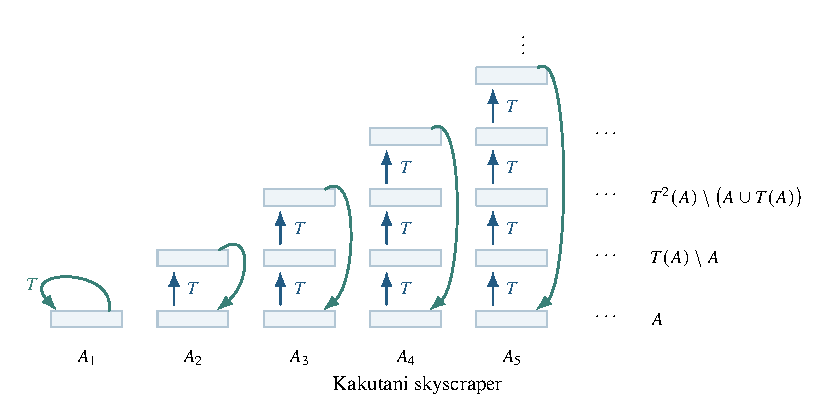
\includegraphics[width=.92\textwidth]{lecture5-fig-01.pdf}
 \FigureTag{L5.1}{fig:lecture5-fig-01}
\end{figure}

\paragraph{Description.}
The ground floor represents $A$ as a disjoint union of sets $\{A_k\}_{k\geq1}$. By definition, points in $A_2$ travel to some set before returning to $A$. The first floor consists of the sets $A_2$ onwards lifted to a set beyond $A$; the second floor is obtained similarly, and the $n$th floor inductively. $T_A$ takes points in $A_3$, for instance, on a ride to all the floors above it and lands on $A$.

\begin{remark}
Poincar\'e recurrence is basically saying that the ground floor has $\{A_k\}_{k\geq1}$ almost everywhere, and hence the tower above it. Ergodicity of $T$ tells you that every point of $X$ belongs to some floor of the skyscraper, as $\mu(A)>0$.
\end{remark}

% Source page 5
\setcounter{theorem}{16}\begin{theorem}[Expected Return Time, due to Kac]\label{thm:l5-kac}
Let $(X,\mathcal B,\mu,T)$ be an invertible ergodic system. If $\mu(A)>0$, then
\[
 \int_A r_A\,d\mu=1.
\]
In other words, the expected return time is
\[
 \frac1{\mu(A)}\int_A r_A\,d\mu=\frac1{\mu(A)}.
\]
\end{theorem}
\Needspace{5\baselineskip}
\begin{proof}
Since $T$ is invertible, ergodicity of $T$ implies ergodicity of $T^{-1}$. As we know, $\mu\bigl(\bigcup_{n\geq1}T^n(A)\bigr)=1$, so the skyscraper contains almost all of $X$. Thus, summing up tower-wise,
\[
\begin{aligned}
 1=\mu(X)
 &=\sum_{n\geq1}\mu\bigl(A_n\sqcup T(A_n)\sqcup\cdots\sqcup T^{n-1}(A_n)\bigr)\\
 &=\sum_{n\geq1}n\mu(A_n)=\int_A r_A\,d\mu,
\end{aligned}
\]
as $\sum_{k=1}^n k\chi_{A_k}\nearrow r_A$.
\end{proof}
Therefore, the bigger the set, the sooner the points will return. In particular, if $\mu(A)>\frac12$, then the expected return time is less than $2$.

\setcounter{theorem}{17}\begin{theorem}[Rokhlin's Tower Decomposition]\label{thm:l5-rokhlin}
In the setting of Theorem~\href{https://codezen1729.github.io/math-blog/\#/post/return-times-kakutani-skyscrapers-and-rokhlin-towers}{17}, suppose that $\mu(\{x\})=0$ for all $x\in X$, i.e. $\mu$ is nonatomic. Then for every $n\geq1$ and $\varepsilon>0$, there exists $B\in\mathcal B$ such that
\begin{itemize}
 \item $B,T(B),\ldots,T^{n-1}(B)$ are disjoint;
 \item $\displaystyle\mu\left(\bigsqcup_{k=0}^{n-1}T^k(B)\right)>1-\varepsilon$.
\end{itemize}
\end{theorem}

% Source page 6

This decomposition is usually called a \emph{Rokhlin tower of height $n$ with base $B$ and residual set of size $\varepsilon$}.

This sort of brings us to the end of our discussion on measure-preserving systems. Let us stop by stating things to look forward to.

% Source page 8
In our brief five lectures we have encountered two fundamental questions:
\begin{enumerate}
 \setcounter{enumi}{0}\item The problem of decomposing the state space into ergodic components.
 \setcounter{enumi}{1}\item The problem of classifying measure-preserving systems.
\end{enumerate}
Soon we shall be dealing with these two, and the next thing to look forward to will be the proof of Szemer\'edi's theorem!
% BLOG-CONTENT-END
\end{document}
